\documentclass[12pt]{article}
\usepackage[swedish]{babel}
\usepackage[version=4]{mhchem}
\usepackage{amsmath}
\usepackage[swedish]{varioref}
\usepackage{hyperref}
\hypersetup{
    colorlinks=true,
    linkcolor=black
}
\usepackage[swedish]{cleveref}
\usepackage{amsthm}
\usepackage{cancel}
\usepackage{float}
\usepackage{array}
\usepackage{enumitem}
\renewcommand{\labelitemii}{$\circ$}
\usepackage[margin=2.5cm]{geometry}
\usepackage{pgf}
\usepackage{tikz}
\usepackage{graphicx}
\usetikzlibrary{bending}
\usetikzlibrary{calc}
\usetikzlibrary{animations}
\usetikzlibrary{babel}

\theoremstyle{definition}
\newtheorem{exm}{Exempel}

\title{Sammanfattning - Kemi 2 \\ Blackebergs Gymnasium}
\author{Marcell Ziegler - NA21D}



\begin{document}
    \begin{titlepage}
        \maketitle
        \vfill
        \begin{center}
            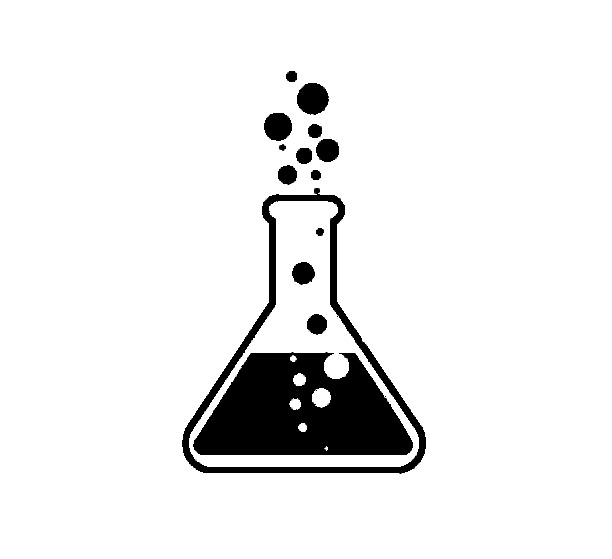
\includegraphics[width=0.8\textwidth]{title.png}
        \end{center}
        \vfill
        \begin{center}
            \textbf{OBS!} Alla siffror/refenser som verkar/borde vara länkar är \\ antagligen länkar, tryck gärna!
        \end{center}
    \end{titlepage}

    \tableofcontents

    \newpage
    \flushbottom
    
    \part{Kemisk jämvikt}
    En jämvikt är en kemisk reaktion som går åt båda håll. När ett så kallat \emph{jämviktstillstånd} är uppnått har reaktionen samma reaktionshastighet dvs. att den ''går lika snabbt'' åt båda håll. Detta medför att förhållandet mellan reaktanter och produkter förblir densamma. Egentligen är alla reaktioner jämvikter men vissa är så pass förskjutna åt ena hållet att de betraktas som fullständiga. Tecknet $\ce{<=>}$ används för att visa jämvikt, se följande exempel:
    \begin{equation*}
        \ce{HCl + H2O <=> H3O+ + Cl-}
    \end{equation*}

    \input{chapters/jämviktskonstant.tex}
    \setcounter{exm}{0}
    
    \input{chapters/förskjutning.tex}
    \setcounter{exm}{0}

    \part{Reaktionshastighet}
    Reaktionshastighet är en annan central del av denna kurs. Kortfattat är det hur snabbt en reaktion sker uttryckt i $\mathrm{\left[\frac{Molar}{Sekund} = \frac{M}{s} = \frac{mol}{dm^3 \cdot s}\right]}$. Detta ger oss formeln 
    \begin{equation*}
        v = \frac{\Delta C}{\Delta t} 
    \end{equation*}
    där $v = \text{reaktionshastighet i } \mathrm{M/s}$. Om man av någon anledning hade velat teckna en funktion $C(t)$ hade $v = C'(t) = \frac{dC}{dt}$ gällt.

    \section{Påverkande faktorer}
Reaktionshastigheten kan påverkars av många faktorer\footnote{se s. 28--31 i boken}. Här kommer en sammafattning.
\subsection{Bindningar}
Fria joner reagerar nästa omedelbart, exempelvis i fällningar. När detta sker är reaktionen \emph{momentan}. Fri joner har inte några bindningar som måste brytas innan reaktionen kan ske vilket gör det snabbare. Molekyler kommer alltid att reagera långsammare då det tar tid och energi att bryta deras bindningar för reaktionen.

\subsection{Kontaktyta}
Jo större ytan som reaktionen sker på är desto snabbare kommmer den att gå. Detta beror på att de reagerande ämnena måste kollidera för att reaktionen ska ske. Ju mer yta att kollidera på desto fler kollisioner alltså desto snabbare reaktion.

\subsection{Aggregationstillstånd}
Aggregationstillståndet, eller i detta fall hur fritt partiklarna rör sig, kommer ha en stor effekt på reaktionshastigheten. En gas kommer ju ha högst rörlighet, sedan vätskor och sist fasta ämnen. Ju mer partiklarna rör sig desto fler chanser kommer de få att kollidera med varandra och desto snabbare kommer reaktionen att gå.

\subsection{Katalysatorer}
\label{sec:katalysator}
En katalysator är ett ämne som gör en reaktion snabbare eller möjliggör en reaktion som annars är omöjlig utan att själv förbrukas. Den gör detta genom att sänka aktiveringsenergin (\textcolor{red}{\underline{\textbf{\textit{missing reference}}}})av reaktionen. Antingen kommer den att hamna under gränsen för tillgänglig energi vilket möjliggör reaktionen eller så kommer den helt enkelt minska energikravet och öka hastigheten.

\subsection{Koncentration}
En högre koncentration gör partiklarna tätare vilket i sin tur leder till snabbare reaktioner. Detta medför också att tryckförändringar påverkar reaktionshastighet i komprimerbar materia (ex. gaser).

\section{Reaktionens energi}

\subsection{Endoterm och exoterm}
En reaktion kan vara endo- eller exoterm. En endoterm reaktion kräver energi medan en exoterm reaktion avger ett överskott av energi\footnote{se s. 32--33 i boken}.

\subsection{Entalpi}
    
\begin{figure*}[h]
    \centering
    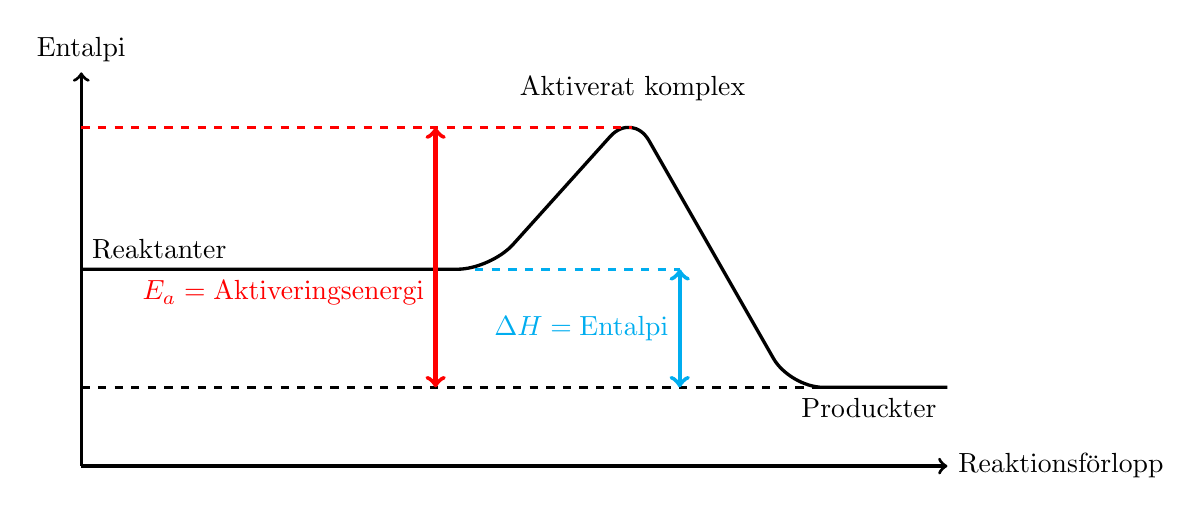
\begin{tikzpicture}
        \draw [->,very thick] (0,0) -- (0,5) node[anchor=south] {Entalpi};
        \draw [->,very thick] (0,0) -- (11,0) node[anchor=west] {Reaktionsförlopp};
        \draw [very thick,rounded corners=12pt] (0,2.5) node[anchor=south west] {Reaktanter} -- (5.2,2.5) -- (7, 4.5) node[anchor=south] {Aktiverat komplex} -- (9,1) -- (11,1) node[anchor=north east] {Produckter};
        \draw [dashed,very thick,color=red] (0,4.3) -- (7,4.3);
        \draw [dashed,very thick] (0,1) -- (10.5,1);
        \draw [ultra thick,<->,color=red] (4.5,1) -- (4.5,2.5) node[anchor=north east] {$E_a = \text{Aktiveringsenergi}$} -- (4.5,4.3);
        \draw [very thick, dashed, color=cyan] (5,2.5) -- (7.6,2.5);
        \draw [ultra thick, <->, color=cyan] (7.6,1) -- (7.6,1.75) node[anchor=east] {$\Delta H =\text{Entalpi}$} -- (7.6,2.5);
    \end{tikzpicture}
\end{figure*}
    \setcounter{exm}{0}

    \part{Syror och Baser}
    Syror och baser är två av de tviktigaste typerna av ämnen för denna kurs. En syra är ett ämne som tar upp en $\ce{H+}$ jon när den reagerar med $\ce{H2O}$ medan en bas avger en jon instället. Minnesregeln är ''BUSA'': ''\underline{\textbf{B}}aser \underline{\textbf{U}}pptar, \underline{\textbf{S}}yror \underline{\textbf{A}}vger''.

    Ett annat viktigt kännetecken är att alla vattenlösningar kommer innehålla \emph{oxoniumjoner} ($\ce{H3O+}$) och \emph{hydroxidjoner} ($\ce{OH-}$). Förhållandet mellan dessa kommer vara lite olika beroende på lösningen. I en neutral lösning kommer de att vara lika många av varje, i syrliga lösningar finns fler $\ce{H3O+}$ och i basiska lösningar finns det fler $\ce{OH-}$.

    \section{Protolys}

Protolys\footnote{se s. 60 i boken}---från \emph{proto} för proton och forngrekiskans \emph{lúsis} för lossa---innebär att det sker ett utbyte av en eller flera protoner ($\ce{H+}$ joner). Som angivet ovan kommer syror lossa en proton och baser ta emot en.
\begin{exm}
    Låt en syra A som innehåller en väteatom H reagera med vatten. Detta kallas också att den \emph{protolyseras} med vatten:
    \begin{center}
        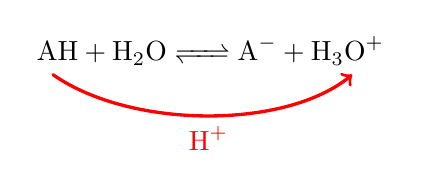
\begin{tikzpicture}
            \node at (0,0) {$\ce{AH + H2O <=> A- + H3O+}$};
            \draw[very thick, color=red, ->, line cap=round] (-2,-0.3) .. controls (-1,-1) and (1,-1) .. node[anchor=north] {$\ce{H+}$} (1.8,-0.3);
        \end{tikzpicture}
    \end{center}
    Något mycket liknande sker när en bas B protolyseras:
    \begin{center}
        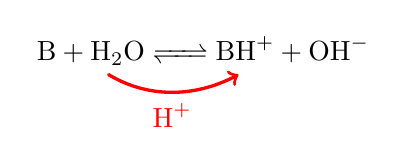
\begin{tikzpicture}
            \node at (0,0) {$\ce{B + H2O <=> BH+ + OH-}$};
            \draw[very thick, color=red, ->, line cap=round] (-1.2,-0.3) .. controls (-0.7,-0.6) and (-0.1,-0.6) .. node[anchor=north] {$\ce{H+}$} (0.45,-0.3);
        \end{tikzpicture}
    \end{center}
\end{exm}

\subsection{Svaga/starka syror och baser}
Man säger att en syra eller en bas kan antingen vara stark eller svag\footnote{se s. 63 samt uppgift 3:29--3.20 i boken}. Detta har faktiskt ingen korrelation med hur mycket den förändrar pH utan det betecknar om reaktionen är fullständig. En syra/bas som protolyseras helt när den placeras i vattelösning kallas stark och alla andra är svaga.

\section{pH och pOH}

Dessa är ett mått på hur syrligt eller basiskt en lösning är. pH är absolut standard med det finns anvädningar för pOH också. Skalan är logaritmisk med bas 10 och går från ca -1 till ca 14. Definitionen för de två storheterna är:
\begin{align*}
    \mathrm{pH} &= -\log_{10}{\ce{[H3O+]}} \\
    \mathrm{pOH} &= -\log_{10}{\ce{[OH^-]}}
\end{align*}
Ju större pH är desto mer basiskt och ju mindre den är desto mer syrligt. En neutral lösning har pH 7, då är $\ce{[H3O+] = [OH^-]}$. För att beräkna den ena från den andra vet vi även detta samband:
\[
    \mathrm{pH + pOH} = 14
\]

\section{Syra- och baskonstanten}
Mycket likt jämviktskonstanten $K$ finns den en så kallad \emph{syrakonstant} $K_a$ och en \emph{baskonstant} $K_b$. Dessa beskriver hur fullständig en syra/bas protolyseras. Dessa värde existerar även för amfolyter---ämnen som är både syra och bas---och bestämmer då om de hellre reagerar som syra eller bas. Dessa värde är som $K$ för för protolysen men man bortser från [$\ce{H2O}$] alltså ser det ut såhär:
\begin{align*}
    K &= \frac{\mathrm{[Bas]} \cdot [\ce{H3O+}]}{\cancel{\ce{[H2O]}} \cdot \mathrm{[Syra]}} \\
    K_a &= \frac{\mathrm{[Bas]} \cdot [\ce{H3O+}]}{\mathrm{[Syra]}} 
\end{align*}
för en syra och följande för en bas:\begin{align*}
    K &= \frac{\mathrm{[Syra]} \cdot [\ce{OH^-}]}{\cancel{\ce{[H2O]}} \cdot \mathrm{[Bas]}} \\
    K_b&= \frac{\mathrm{[Syra]} \cdot [\ce{OH^-}]}{\mathrm{[Bas]}} 
\end{align*}

\subsection{Räkna med syra- och baskonstanten}
Man räknar på dessa konstanter ungefär som man räknar med $K$ (se \vref{sec:räknak}). Skillnaden är att du kommer veta $K_a \text{ eller } K_b$ i förväg från en tabell. Du kan sedan utnyttja detta för att ställa upp jämvikten med tidigare angivna tabeller för att sedan beräkna $\ce{[H3O+] \text{ eller } [OH^-]}$ i en lösning som i sin tur kan leda till pH. Detta är viktigt för att det fungerar även för svaga syror och baser

\subsection{Joner som syra eller bas}
Ibland kan vissa joner från olika salter agera som syror eller baser. Man kan bestämma detta genom att dela upp saltet i dess beståndsdelar. Efter denna uppdelning kan man kolla upp $K_a$ och $K_b$ för dessa joner och avgöra om de reagerar som syra/bas och vilket av dem isåfall. Därefter är logiken för pH exakt samma som för ''vanliga'' syror.

\section{Titrering}
Titrering är ett sätt att ta reda på olika egenskaper hos en syra eller en bas. Man kan exempelvis beräkna mängden kristallvatten, pH, $K_a$ eller $K_b$ från en titrering. Processen går ut på att man placerar någonting i en vattenlösning och i denna lösningen droppar man in en annan med en byrett. 
\begin{figure*}[h]
    \centering
    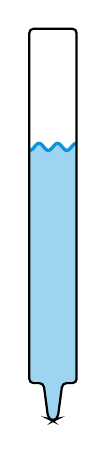
\begin{tikzpicture}[scale=1.5, every node/.style=[scale=1.5]]
        \fill[thick, domain=-0.2:0.2, color=cyan!80!blue, fill opacity=0.4] (-0.2,-3) -- plot [samples=50] (\x, {0.03*sin((40*\x) r)-1}) [rounded corners=1.5pt] -- (0.2,-3)  -- (0.08,-3) -- (0.04,-3.3) -- (0,-3.32) -- (-0.04,-3.3) -- (-0.08,-3) -- cycle;
        \draw[very thick, domain=-0.2:0.2, color=cyan!80!blue] plot [samples=50] (\x, {0.03*sin((40*\x) r)-1});
        \draw[thick, rounded corners=1.5pt] (-0.2,0) -- (-0.2, -3) -- (-0.08,-3) -- (-0.04,-3.3) -- (0,-3.32) -- (0.04,-3.3) -- (0.08,-3) -- (0.2,-3) -- (0.2, 0) -- cycle;
    \end{tikzpicture}
\end{figure*}
\end{document}